\documentclass{article}
\usepackage{graphicx} % Required for inserting images
\usepackage{placeins}
\usepackage{amsmath,amssymb}
\usepackage[dvipsnames]{xcolor}
\usepackage{hyperref}
\usepackage[most]{tcolorbox}

\usepackage{tikz}
\usetikzlibrary{arrows.meta,fit,positioning,shapes,calc}

\usepackage{listings}

\newtcolorbox{keybox}[1]{
  colback=blue!3,
  colframe=MidnightBlue!60!black,
  title=\textbf{#1},
  fonttitle=\small,
  breakable,
  sharp corners,
  boxrule=0.6pt
}

\newtcolorbox{warningbox}[1]{
  colback=red!3,
  colframe=red!60!black,
  title=\textbf{#1},
  fonttitle=\small,
  breakable,
  sharp corners,
  boxrule=0.6pt
}

\newtcolorbox{examplebox}[1]{
  colback=ForestGreen!4,
  colframe=ForestGreen!55!black,
  title=\textbf{#1},
  fonttitle=\small,
  breakable,
  sharp corners,
  boxrule=0.6pt
}

\lstdefinestyle{tutorialcode}{
  basicstyle=\ttfamily\footnotesize,
  breaklines=true,
  columns=fullflexible,
  keepspaces=true,
  showstringspaces=false,
  frame=single,
  framerule=0.2pt,
  rulecolor=\color{black!30},
  backgroundcolor=\color{black!2}
}
\lstset{style=tutorialcode}

\title{Intelligence via generation and selection: A tutorial on reinforcement learning with LLMs and tools}
\author{Nando de Freitas and Everyone}
\date{\today}


% Macros for consistent coloured notation.
\newcommand{\colsym}[2]{\ensuremath{\textcolor{#1}{\boldsymbol{#2}}}}

% Existing RL symbols.
\newcommand{\action}{\colsym{red}{a}}
\newcommand{\obs}{\colsym{ForestGreen}{o}}
\newcommand{\reward}{\colsym{purple}{r}}
\newcommand{\nextaction}{\colsym{red}{a'}}
\newcommand{\nextobs}{\colsym{ForestGreen}{o'}}
\newcommand{\params}{\colsym{blue}{\theta}}
\newcommand{\return}{\ensuremath{\textcolor{cyan}{\boldsymbol{R}}}}

% Policy and trajectory notation.
% Important: the policy \pi and the parameters \theta are kept separate.
% We write \pi(a \mid o ; \theta), not \pi_\theta(a \mid o).
\newcommand{\policy}{\colsym{MidnightBlue}{\pi}}
\newcommand{\trajectory}{\colsym{teal}{\tau}}

% Optimisation and learning-dynamics symbols.
\newcommand{\loss}{\ensuremath{\textcolor{MidnightBlue}{\mathcal{L}}}}
\newcommand{\perf}{\ensuremath{\textcolor{MidnightBlue}{J}}}
\newcommand{\learnfield}{\colsym{RoyalBlue}{G}}
\newcommand{\stepsize}{\colsym{cyan}{\alpha}}

% Policy-gradient demo symbols.
\newcommand{\advantage}{\colsym{Orange}{A}}
\newcommand{\refpolicy}{\ensuremath{\textcolor{MidnightBlue}{\boldsymbol{\pi}_{\mathrm{ref}}}}}
\newcommand{\klcoef}{\colsym{Mahogany}{\beta}}
\newcommand{\shapedreward}{\ensuremath{\widetilde{\reward}}}

% Dynamical-systems and game-theory symbols.
\newcommand{\potential}{\colsym{MidnightBlue}{\Phi}}
\newcommand{\lyap}{\colsym{Orange}{V}}
\newcommand{\hamiltonian}{\colsym{Mahogany}{H}}
\newcommand{\rotfield}{\colsym{BrickRed}{\Omega}}
\newcommand{\utility}{\colsym{purple}{u}}
\newcommand{\player}{\colsym{BrickRed}{i}}
\newcommand{\discount}{\colsym{cyan}{\gamma}}

% Value-function notation, kept distinct from Lyapunov V by colour.
\newcommand{\valfn}{\colsym{cyan}{V}}
\newcommand{\qfn}{\colsym{cyan}{Q}}

% General mathematical helpers.
\newcommand{\E}{\mathbb{E}}
\newcommand{\dd}{\mathrm{d}}
\newcommand{\norm}[1]{\left\lVert #1 \right\rVert}


\begin{document}

\maketitle


\section{Intelligence via generation and selection}

The central theme of this note is that intelligent systems become powerful when they can both \emph{generate} candidate behaviours and \emph{select} among them. This is a useful way to connect several traditions. In philosophy, \href{https://en.wikipedia.org/wiki/Agency_(philosophy)}{agency} is the capacity of an actor to act in an environment; in AI, an \href{https://en.wikipedia.org/wiki/Intelligent_agent}{intelligent agent} is often described as something that perceives an environment, acts autonomously to achieve goals, and may improve through learning.

\href{https://en.wikipedia.org/wiki/Supervised_learning}{Supervised learning} corresponds to the most trivial form of imitation: \emph{mimicking}. It uses \href{https://en.wikipedia.org/wiki/Maximum_likelihood_estimation}{maximum likelihood}--the way we pretrain and SFT LLMs--to map states of the world, such as text questions, to actions, such as text answers. We call such mappings policies. In supervised learning, the teacher demonstrates what to do, but does not grade. Hence the student is only as good as the demonstrations, and good expert data is expensive.

As an aside, there are very powerful ways of doing supervised learning with very general experts: next-step prediction, denoising, and reconstruction. This is basically how pretraining of LLMs works, and also how diffusion, flow matching, and autoencoder-style methods work in multimodal perception and generation. These are often called \href{https://en.wikipedia.org/wiki/Self-supervised_learning}{self-supervised} or unsupervised because the target is extracted from the data itself rather than supplied as an external human label.

\href{https://en.wikipedia.org/wiki/Reinforcement_learning}{Reinforcement learning} (RL), on the other hand, is about \emph{selective imitation}. The agent does not have to imitate every piece of behaviour in the data. Instead, it can use rewards, value functions, reward models, critics, tests, or other evaluators to decide which behaviours are worth reinforcing and which behaviours should be ignored. In this sense RL can exploit huge amounts of cheap, noisy, or suboptimal data generated by many agents. We do not imitate everything our parents do; we select the useful bits and try to forget the rest.


Supervised learning says: imitate the demonstrated action. RL says: generate or collect candidate trajectories, evaluate them, and put more probability mass on the candidates that lead to better outcomes. 
The learning signal is not just ``what action did the teacher take?'' but ``which actions led to high return?''. 

RL is also about self-improvement. Agents \emph{generate} data by acting in the environment. They can learn from their own successes and mistakes, as well as from a replay buffer containing data from other agents. When we use reward signals to construct selection mechanisms--for example, rank many sampled answers and train only on the best half--the agent can start learning from its own data and self-improve. 

Moreover, because an action \action{} changes the environment, interaction produces interventional knowledge. In causal notation, the agent is trying to learn what happens under an intervention, that is \(P(\nextobs\mid \operatorname{do}(\action),\obs)\), not merely what tends to co-occur in passive data. For background see this discussion on \href{https://en.wikipedia.org/wiki/Causal_model}{causal models}. RL researchers omit writing the do operator explicitly, but it would be reckless to assume the world model is an observational model \(P(\nextobs\mid \action,\obs)\). It is an interventional model. The actions of an agent behaving in an environment are interventions, not observations.

The price RL pays is that interventions can be expensive, slow, or dangerous. For this reason, \emph{agents can use mental models or external tools--simulators, test suites, calculators, web browsers, theorem provers, code interpreters--to run cheaper experiments before acting in the real world.} Incidentally, I haven't heard anyone proposing to use tools as world models, but this is indeed viable and I believe a great argument for RL. This is not merely an implementation trick. The \href{https://en.wikipedia.org/wiki/Extended_mind_thesis}{extended mind thesis} of Clark and Chalmers argues that cognition can extend into tools and the surrounding environment, and Dennett's \href{https://en.wikipedia.org/wiki/The_Intentional_Stance}{intentional stance} explains why treating a system as a rational, goal-directed agent can be a useful predictive strategy. Modern tool-using LLM agents make these old philosophical ideas feel very concrete.

In \href{https://en.wikipedia.org/wiki/The_Beginning_of_Infinity}{\emph{The Beginning of Infinity}}, David Deutsch makes a strong case for knowledge growth through conjectures and criticism: generate explanations, criticise them, and keep the ones that survive. Darwin's theory of \href{https://en.wikipedia.org/wiki/Natural_selection}{natural selection} is the biological ancestor of this view: variation generates candidates, and selection preserves the ones that survive and reproduce. Darwin's \href{https://en.wikipedia.org/wiki/On_the_Origin_of_Species}{\emph{On the Origin of Species}} and Deutsch's book are therefore useful background reading for this generation-and-selection perspective.

RL has roots in psychology. In \href{https://en.wikipedia.org/wiki/Operant_conditioning}{operant conditioning}, voluntary behaviours are modified by association with rewards or aversive stimuli: reinforcement increases a behaviour, while punishment or extinction decreases it. \href{https://en.wikipedia.org/wiki/B._F._Skinner}{B. F. Skinner} developed behaviour analysis and used operant conditioning to study how consequences shape future behaviour. I highly recommend reading Skinner's books.

There is also a deep economic lineage. \href{https://en.wikipedia.org/wiki/Theory_of_Games_and_Economic_Behavior}{von Neumann and Morgenstern} helped formalise decision theory and expected utility. The \href{https://en.wikipedia.org/wiki/Von_Neumann\%E2\%80\%93Morgenstern_utility_theorem}{von Neumann--Morgenstern utility theorem} says that, under suitable axioms, rational choice under uncertainty can be represented as maximising expected utility. \href{https://en.wikipedia.org/wiki/Subjective_expected_utility}{Savage's subjective expected utility} framework then made uncertainty personal: the agent combines its own probabilities with its own utility function. Modern RL inherits this optimisation language, replacing utility with reward and expected utility with value or expected return.


Silver, Singh, Precup, and Sutton's \href{https://www.sciencedirect.com/science/article/pii/S0004370221000862}{\emph{Reward is Enough}} hypothesis says that intelligence and its associated abilities can be understood as serving reward maximisation. That view is coherent and inspiring, but it assumes that the reward signal is the right selection mechanism. In real systems the desired objective may be hard to specify, and agents may exploit proxy rewards in unintended ways--the classic \href{https://en.wikipedia.org/wiki/Reward_hacking}{reward hacking} or specification-gaming problem. RL is therefore not just about maximising the reward \reward{}. It also involves designing, learning, auditing, and stress-testing the selection rule. I expand on this in the last section of this tutorial.


Finally, reward-maximising agency is not the only route to purposeful behaviour. Pedro Ortega's \href{https://adaptiveagents.org/universal_ai_as_imitation}{\emph{Universal Artificial Intelligence as Imitation}} gives a complementary account based on interaction, imitation, and first-person updating. In that view, an agent's actions are choices that set up evidence, while the world's observations are the evidence used for learning. Reward can still appear as one kind of observation, but purpose does not have to be defined first as a scalar reward. This is a useful reminder for modern AI: agents may learn causal knowledge not only by maximising rewards, but also by imitating structured interactions, using tools, following protocols, absorbing norms, and learning what tends to happen after their own interventions.


\section{RL systems}

An \emph{agent} is an entity that perceives its environment, takes actions autonomously to achieve goals, and may improve its performance through reinforcement learning or teaching. Agents can have internal goals (inferred subgoals, and the desire to observe more, learn more, or control more -- yes, we should be thinking safety here!) or external goals either specified as reward functions or as feedback reward signals. Figure~\ref{fig:rl-framework} shows the main ingredients of RL.
\begin{figure}[h]
    \centering
    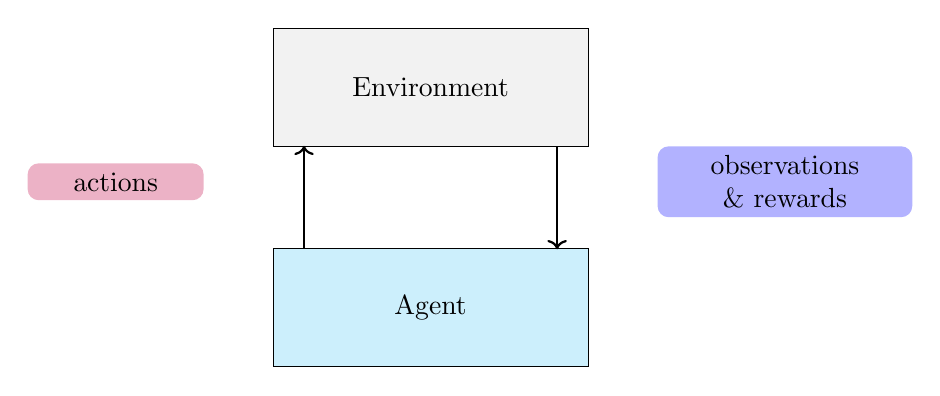
\begin{tikzpicture}
        % Draw Environment
        \node[draw, fill=gray!10, minimum width=4cm, minimum height=1.5cm] (env) at (0,2.2) {Environment};
       
        % Draw Agent
        \node[draw, fill=cyan!20, minimum width=4cm, minimum height=1.5cm] (agent) at (0,-.6) {Agent};
       
       % Draw separate arrows
        \draw[->, thick] (agent.north west) ++(0.4,0) -- ++(0,1.3) node[midway, right] {};
        \draw[->, thick] (env.south east) ++(-0.4,0) -- ++(0,-1.3) node[midway, left] {};
           
        % Labels
        \node[fill=blue!30, text width=3cm, align=center, rounded corners] at (4.5,1) {observations \\ \& rewards};
        \node[fill=purple!30, text width=2cm, align=center, rounded corners] at (-4,1) {actions};
    \end{tikzpicture}
    \caption{Reinforcement Learning entities.}
    \label{fig:rl-framework}
\end{figure}


An agent could be a multimodal neural net that interacts with a user (its environmnent) to empower the user with personalised education (the goal). The more the agent observes, the easier it is for the agent to create a personalised curriculum to assist the user.

As shown in Figure~\ref{fig:distributed-rl}, modern distributed RL systems are broken down into two components: Actors and Learners. Each actor interacts with the environment by generating actions with a network known as the \emph{policy}. The actors also gather rewards and observations from the environment. The data collected are added to a common replay memory. The learner samples data from the replay memory and uses it to update the policy network. After updating the network, the weight checkpoints need to be sent to each actor. It is important when designing such systems to measure the duration of each operation, measure the bandwidth of each communication link, and so on. This demands precise engineering and comprehensive measurements and ablations.

In language, the actors are chatbot agents and the environments are people. The data from each chat is then sent to a replay memory for learning. Typically the learner may require more storage and compute than the actors. It is important to know the costs of inference at the actors and the costs of learning. In some settings, these costs allow for the agent to learn on-policy, in which case the replay memory simply acts as a buffer. Note that this is typically asynchronous because different actors work at different speeds. On the other hand, if the data is not gathered fast enough, it may be necessary to replay old examples to update the policy. This is the off-policy setting. Here, it is important to correct for the fact that the model is being learned with stale data. We will see later that people often introduce importance weights and other mechanisms to correct for this.

Finally, sometimes it is possible to learn the policy from a big replay data alone. This is known as off-line RL or batch RL. Off-line RL is better than supervised learning because it includes selection mechanisms, but it is of course not as good as on-line RL because it lacks direct generation of actions on environments. However, off-line RL can be really useful and allow for learning in situations where interaction is either costly or dangerous.





\begin{figure}[ht!]
\centering
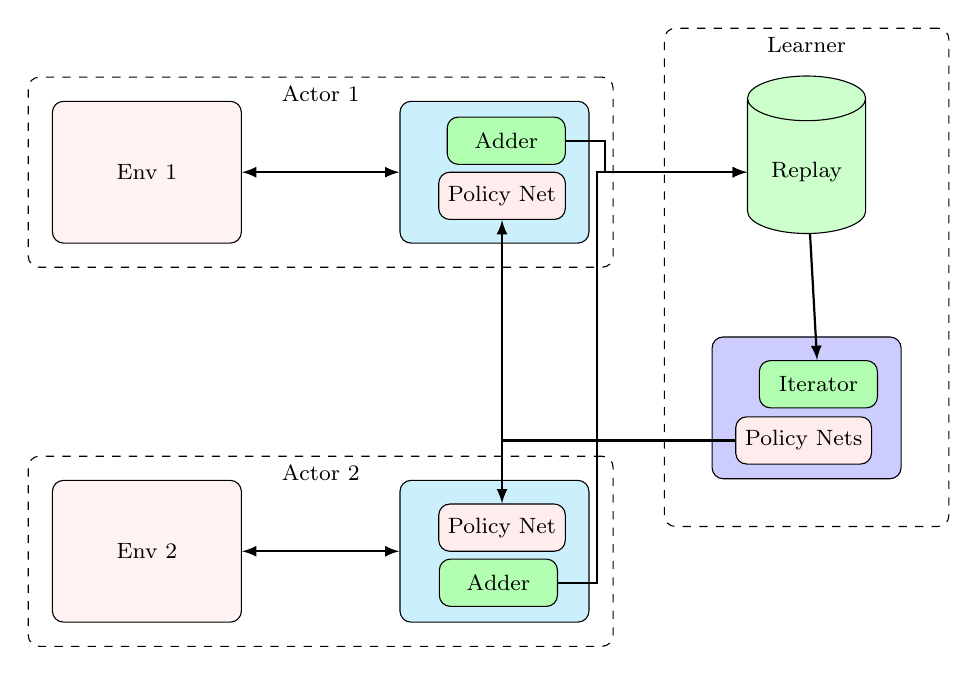
\begin{tikzpicture}[
  font=\footnotesize,
  >=latex,
  % Styles
  dashedbox/.style={draw,dashed,inner sep=0.3cm,rounded corners},
  module/.style={draw,rectangle,rounded corners,minimum width=2.4cm,minimum height=1.8cm,align=center},
  smallmodule/.style={draw,rectangle,rounded corners,minimum width=1.5cm,minimum height=0.6cm,align=center},
  arrowstyle/.style={->,thick},
  ]

%--- Machine 3 box --------------------------------------------------
% Environment
\node[module, fill=pink!20] (env3) {Env 1};

% Actor
\node[module, fill=cyan!20, right=2cm of env3] (actor3) { };

% Sub-boxes inside Actor on Machine 3
\node[smallmodule, fill=pink!30, anchor=south east, xshift=-0.3cm, yshift=0.3cm]
  (pol3) at (actor3.south east) {Policy Net};
\node[smallmodule, fill=green!30, anchor=north east, xshift=-0.3cm, yshift=-0.2cm]
  (add3) at (actor3.north east) {Adder};

% Arrows between Env and Actor
\draw[<->,thick] (env3) -- (actor3);

% Dashed bounding box labeled "Machine 3"
\node[dashedbox, fit=(env3)(actor3), label={[below]Actor 1}] (machine3) {};

%--- Machine 2 box --------------------------------------------------
% Environment
\node[module, fill=pink!20, below=3cm of env3] (env2) {Env 2};

% Actor
\node[module, fill=cyan!20, right=2cm of env2] (actor2) { };


% Sub-boxes inside Actor on Machine 2
\node[smallmodule, fill=pink!30, anchor=north east, xshift=-0.3cm, yshift=-0.3cm]
  (pol2) at (actor2.north east) {Policy Net};
\node[smallmodule, fill=green!30, anchor=south east, xshift=-0.4cm, yshift=0.2cm]
  (add2) at (actor2.south east) {Adder};

% Arrows between Env and Actor
\draw[<->,thick] (env2) -- (actor2);

% Dashed bounding box labeled "Machine 2"
\node[dashedbox, fit=(env2)(actor2), label={[below]Actor 2}] (machine2) {};

%--- Machine 1 box --------------------------------------------------
% "Replay" as a cylinder
\node[
  cylinder,
  shape border rotate=90,
  draw,
  fill=green!20,
  minimum height=2cm,
  minimum width=1.5cm,
  aspect=0.5,
  right=2cm of actor3
] (replay) {Replay};

% Learner
\node[module, fill=blue!20, below=1.3cm of replay] (learner) { };

% Sub-boxes inside Learner
\node[smallmodule, fill=pink!30, anchor=north west, xshift=0.3cm, yshift=0.8cm]
  (netL) at (learner.south west) {Policy Nets};
\node[smallmodule, fill=green!30, anchor=north east, xshift=-0.3cm, yshift=-0.3cm]
  (iter) at (learner.north east) {Iterator};

\node[
  dashedbox,
  fit=(replay)(learner),
  % Add extra spacing inside the bounding box
  inner xsep=0.6cm,
  inner ysep=0.6cm,
  label={[below]Learner}
] (machine1) {};


%--- Inter-machine connections --------------------------------------
% Arrows from each Actor’s Adder to Replay
\draw[arrowstyle] (add3.east) -- ++(0.5,0) |- (replay.west);
\draw[arrowstyle] (add2.east) -- ++(0.5,0) |- (replay.west);

% Arrow from Replay to Iterator (inside Learner)
\draw[arrowstyle] (replay) -- (iter);

% Arrows from Learner's Networks back to each Actor's Networks
\draw[arrowstyle] (netL.west) -| (pol3.south);
\draw[arrowstyle] (netL.west) -| (pol2.north);

\end{tikzpicture}
\caption{Distributed RL setup with two actors
         and a central replay buffer and learner.}
\label{fig:distributed-rl}
\end{figure}






\section{The many types of RL problems}



\begin{figure}[h!]
    \centering      
    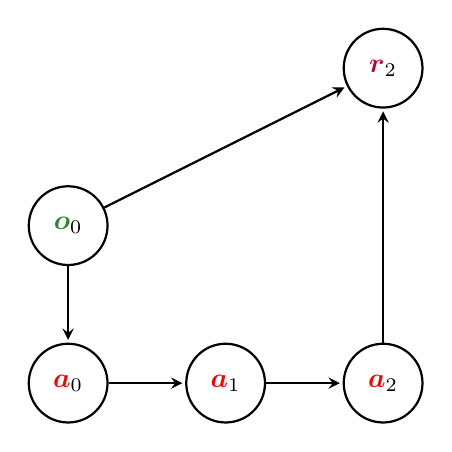
\begin{tikzpicture}[->,>=stealth,shorten >=1pt,auto,node distance=2cm,thick]
        \tikzstyle{state} = [circle, draw, minimum size=1cm, text centered]
        \tikzstyle{state2} = [circle, draw=white, minimum size=1cm, text centered]

        % Nodes
        \node[state] (o0) {\obs$_0$};
        \node[state, below of=o0] (a0) {\action$_0$};
        \node[state2, right of=o0] (o1) {};
        \node[state, below of=o1] (a1) {\action$_1$};
        \node[state2, right of=o1] (o2) { };
        \node[state, below of=o2] (a2) {\action$_2$};
        \node[state, above of=o2] (r2) {\reward$_2$};

        % Edges
        \path (o0) edge (r2);
        \path (o0) edge (a0);
        \path (a0) edge (a1);
        %\path (o1) edge (o2);
        %\path (o1) edge (a1);
        \path (a1) edge (a2);
        %\path (o2) edge (a2);
        %\path (a2) edge (o2);
        \path (a2) edge (r2);
        %\path (r2) edge [bend right] (o2);
    \end{tikzpicture}  \hspace{.8cm}
        \begin{tikzpicture}[->,>=stealth,shorten >=1pt,auto,node distance=2cm,thick]
        \tikzstyle{state} = [circle, draw, minimum size=1cm, text centered]
        \tikzstyle{state2} = [circle, draw=white, minimum size=1cm, text centered]

        % Nodes
        \node[state] (o0) {\obs$_0$};
        \node[state, below of=o0] (a0) {\action$_0$};
        \node[state, above of=o0] (r0) {\reward$_0$};
        \node[state, below of=o1] (a1) {\action$_1$};
        \node[state, above of=o1] (r1) {\reward$_1$};
        \node[state2, right of=o1] (o2) { };
        \node[state, below of=o2] (a2) {\action$_2$};
        \node[state, above of=o2] (r2) {\reward$_2$};

        % Edges
        \path (o0) edge (r2);
        \path (o0) edge (a0);
        \path (a0) edge (a1);
        \path (a0) edge [bend right]  (r0);
        \path (o0) edge (r1);
        \path (a1) edge [bend right]  (r1);
        \path (o0) edge (r0);
        \path (a1) edge (a2);
        %\path (o2) edge (a2);
        %\path (a2) edge (o2);
        \path (a2) edge (r2);
        %\path (r2) edge [bend right] (o2);
    \end{tikzpicture}  
\vspace{.8cm}
   
    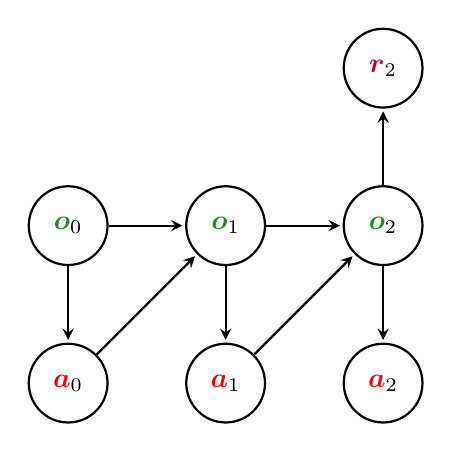
\begin{tikzpicture}[->,>=stealth,shorten >=1pt,auto,node distance=2cm,thick]
        \tikzstyle{state} = [circle, draw, minimum size=1cm, text centered]

        % Nodes
        \node[state] (o0) {\obs$_0$};
        \node[state, below of=o0] (a0) {\action$_0$};
        \node[state, right of=o0] (o1) {\obs$_1$};
        \node[state, below of=o1] (a1) {\action$_1$};
        \node[state, right of=o1] (o2) {\obs$_2$};
        \node[state, below of=o2] (a2) {\action$_2$};
        \node[state, above of=o2] (r2) {\reward$_2$};

        % Edges
        \path (o0) edge (o1);
        \path (o0) edge (a0);
        \path (a0) edge (o1);
        \path (o1) edge (o2);
        \path (o1) edge (a1);
        \path (a1) edge (o2);
        \path (o2) edge (a2);
        %\path (a2) edge (o2);
        \path (o2) edge (r2);
        %\path (r2) edge [bend right] (o2);
    \end{tikzpicture}  \hspace{.8cm}
        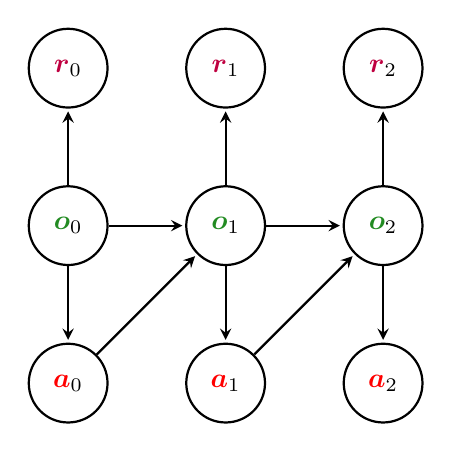
\begin{tikzpicture}[->,>=stealth,shorten >=1pt,auto,node distance=2cm,thick]
        \tikzstyle{state} = [circle, draw, minimum size=1cm, text centered]

        % Nodes
        \node[state] (o0) {\obs$_0$};
        \node[state, below of=o0] (a0) {\action$_0$};
        \node[state, right of=o0] (o1) {\obs$_1$};
        \node[state, below of=o1] (a1) {\action$_1$};
        \node[state, right of=o1] (o2) {\obs$_2$};
        \node[state, below of=o2] (a2) {\action$_2$};
        \node[state, above of=o2] (r2) {\reward$_2$};        
        \node[state, above of=o1] (r1) {\reward$_1$};        
        \node[state, above of=o0] (r0) {\reward$_0$};

        % Edges
        \path (o0) edge (o1);
        \path (o0) edge (a0);
        \path (a0) edge (o1);
        \path (o1) edge (o2);
        \path (o1) edge (a1);
        \path (a1) edge (o2);
        \path (o2) edge (a2);
        %\path (a2) edge (o2);
        \path (o2) edge (r2);
        \path (o1) edge (r1);
        \path (o0) edge (r0);
        %\path (r2) edge [bend right] (o2);
    \end{tikzpicture}

    \caption{Four Markov decision processes (RL models) with finite horizon $T=2$. {\bf [Top left]} This is the setting of \emph{outcome rewards} with LLM, such as deepseek-R1 and chatgpt-o1. The agent generates a string of actions (tokens) and gets a reward at the end. Note that we can group the three actions into a single composite action $\action = (\action_1,\action_2,\action_3)$. {\bf [Top right]} This is the setting of \emph{process rewards} with LLMs. Other than observing a reward at each action step, the agent does not observe any other inputs. {\bf [Bottom left]} This is the tool-use or multi-turn conversation setting. Here, the agent may use a tool $\action_0$ and sense $\obs_1$. Note that the environment can evolve over time, something that we could model with a world-model: $P(\obs_{t+1}|\obs_{t},\action_t)$. A chat agent planning an entire multi-turn conversation with the intent of helping a user, where each turn involves an action by the chat agent (text) and observing the action of the user (text reply) is a good example of this. As the conversation progresses the chat agent adapts and so does the user.
    The game of Go is another example. In both of these, the user is the environment. In truth, if the user is adversarial or manipulative, we are outside the realm of RL and in the world of game theory, but such cases are beyond our scope. {\bf [Bottom right]} Same as previous but with process rewards. }

   
\end{figure}

RL comes in many shapes and forms. It is this variety that makes people work on the problem for years and still be suprised now and then.

To start, many examples of ``finetuning LLMs with RL''
 are \emph{one-step RL problems} (top left of Figure 1). Here, given a prompt the model generates a single action and gets an evaluation. A single action can be a text answer, sketch, speech, any other behaviour signal, or any sequence of tokens. The evaluation is often a \emph{single outcome} reward, e.g. whether the answer is correct.
 
 In a multi-step conversation with a chatbot, the user is the environment and the chatbot the agent. Deciding what to say next, while the user does not provide any inputs, is a one-step RL problem. This is clear in Figure 1 (top left) because the three actions can be easily combined into a single one without destroying the structure of the decision graph. However, planning an entire conversation to achieve a goal at the end, during which both user and chat agent adapt, is a multi-step RL problem (Figure 1, bottom left). This setting could also model a chatbot using tools, e.g. a web browser or slack, to gather information.

RL can involve many steps, where at each step the world changes. As a result, when one gets a reward, one does not know which of the many decisions led to the reward. People call this the \emph{credit assignment problem}. RL, because of the many-steps, is combinatorial and very high-dimensional. Moreover, not knowing the horizon, i.e. the number of decision steps, can create additional trans-dimensional inference complexity. In short, RL is really hard, and the variance of the solutions can be very high. Researchers have invented a series of concepts to keep the variance under check at the expense of introducing bias, including value functions (functions that represent the expected rewards, with some guess as to how to discount future rewards). These concepts are useful in multi-step decision problems, but not always needed for one-step RL.

It is dangerous to import blindly the theory and software of RL methods developed for computer games to the world of language models. Those methods had to deal with asynchronous expensive data generation with game engines and stale replay buffers. Instead, it is important to measure the efficiency of all components in the system and optimize the algorithms for the available hardware and types of interaction.

For tool-use and multi-step assistance, we need multi-step RL for LLMs. However, to do what deepseek-R1 and chatgpt-o1 do, it may suffice to first solve the one-step RL problem, which is slightly simpler. Some of the software, e.g. for policy gradients introduced later in this document, might be very similar for both one-step and multi-step RL, so we may as well try to use a common flexible software framework.

All RL agents self-learn and self-improve. If designed well, they can construct datasets of increasing quality, which in turn lead to policies of increasing quality. This property of RL agents is essential for both performance and for safety. Note that in one-step RL, we repeat the process of solving one-step problems, and the improvements should grow with each iteration.

There can be harder RL cases not addressed here. Sometimes the decision horizon is unknown or infinite, thus increasing the complexity of inference. Moreover, the time steps can be continuous or interrupt-driven. The actions and observations can be a mix of discrete and continuous, e.g. text documents with illustrations, and the reward can combine multiple desirable components. There are also extensions to multi-agents in both collaborative and adversarial settings.

For didactic reasons, we will cover the simplest case first: one-step RL. We will cover the main algorithms, and this will be enough to explain methods such as \href{https://arxiv.org/abs/2501.12948}{deepseek-R1}, \href{https://arxiv.org/abs/2308.08998}{ReST} and \href{https://arxiv.org/abs/2312.06585}{ReST$^{EM}$}. Subsequently, we will address multi-step settings, which allow for tool-use. We will avoid introducing more complexity purposely because the simpler methods might be enough for LLM finetuning.



\section{One-step RL problem formulation}


Many teams, including deepseek-r1 and chatgpt-o1, are trying to maximize the following one-step objective function:
\[
J(\params) = \int r(\action, \obs) \pi_{\params}(\action \mid \obs) P(\obs) \; d\action d\obs
\]

The symbols could for example represent the following:
\begin{itemize}
    \item $\obs \equiv$ question or prompt
    \item $\action \equiv$ answer
    \item $\pi_{\params}(\action \mid \obs) \equiv$ LLM model with parameters $\params$
    \item $r(\action, \obs) \equiv$ evaluation metric or reward
\end{itemize}

That is, we are fine-tuning the LLM over all data strings $(\obs, \action)$. I’m using the integral sign to denote very large discrete sums.


\subsection{Method 1: Policy gradient}

This is what people think of as \emph{on-policy} RL or Reinforce. However, in the one-step case, none of the machinery of Reinforce is needed. This is basic gradient following, and calling it RL is unnecessary. It is said to be on-policy because the policy model that generates the samples is the same as the one being learned.

This approach makes sense when generating the samples is cheaper than learning. That is, when the learner can easily get fresh samples on demand. This seems to be the case with text, but it wasn't the case with expensive game simulation engines, where buffers and replay memories had to be introduced to cache data. The data would then go stale, necessitating off-policy methods, which we will discuss in the following section. For now, we will see how to calculate the gradient of our one-step loss. We will then simply follow the gradient to update the parameters.

Reinforced Self Training \href{https://arxiv.org/abs/2308.08998}{ReST} is a good example of this approach. It can indeed be used for self-improvement, while also staying close to human demonstrations. In ReST the reward is used to rank samples. Subsequently, ReST re-learns the policy unsing only the highest ranked samples.

Let us start the derivation of the policy gradient with the one-step objective:
\[
J(\params) = \int r(\action, \obs) \pi_{\params}(\action \mid \obs) P(\obs) \; d\action d\obs
\]

The gradient is trivial to obtain:
\begin{align*}
\nabla_{\params} J(\params) &= \int r(\action, \obs) \nabla_{\params} \pi_{\params}(\action \mid \obs) P(\obs) \; d\action d\obs \\
&= \int r(\action, \obs) \nabla_{\params} \log \pi_{\params}(\action \mid \obs) \pi_{\params}(\action \mid \obs) P(\obs) \; d\action d\obs
\end{align*}
If we generate (sample) a prompt and solutions from the policy, that is $\action^i \sim \pi_{\text{old}}(\action \mid \obs)$ and $\obs^i \sim P(\obs)$, we can approximate the gradient with Monte Carlo:
\[
\nabla_{\params} J(\params) \approx \frac{1}{N} \sum_{i=1}^N r(\action^i, \obs^i) \nabla_{\params} \log \pi_{\params}(\action^i \mid \obs^i)
\]
This is a necessary baseline when fine-tuning LLMs.


\subsubsection{Improvement 1: Baseline subtraction}

If we subtract the mean of $r$ and replace it with the following reward:
\[
   \reward^i = r(\action^i, \obs^i) - \frac{1}{N} \sum_{j=1}^N r(\action^j, \obs^j)
\]
we don't change the location of the maximum (it is only a constant vertical shift of the loss function), but we reduce the variance. GPT4 can easily prove why the variance is lower! We could also scale the rewards, but the benefit of this isn't clear.

This trick should always be used. Moreover, it is extra useful when the rewards are binary and we require a more continuous gradual feedback signal. We can think of the new reward as the \emph{advantage} of $r$ with respect to the mean baseline.



\subsubsection{Improvement 2: Stay close to a good policy}

We can add a KL term to the loss so it's close to the SFT policy $\pi_{\text{SFT}}(\action \mid \obs)$:
\[
D_{\text{KL}}(\pi_{\params} \Vert \pi_{\text{SFT}}) = \int \pi_{\params}(\action \mid \obs) \log \frac{\pi_{\params}(\action \mid \obs)}{\pi_{\text{SFT}}(\action \mid \obs)} \; d\action
\]

Sample $\action^i \sim \pi_{\params}(\action \mid \obs)$, and use the MC approximation again:
\[
D_{\text{KL}}(\pi_{\params} \Vert \pi_{\text{SFT}}) \approx \frac{1}{N} \sum_{i=1}^N \log \frac{\pi_{\params}(\action^i \mid \obs^i)}{\pi_{\text{SFT}}(\action^i \mid \obs^i)}
\]



The KL can also be estimated by:
\[
D_{\text{KL}}(\pi_{\params} \Vert \pi_{\text{SFT}}) = \int \pi_{\params}(\action \mid \obs) \left[ \log \frac{\pi_{\params}(\action \mid \obs)}{\pi_{\text{SFT}}(\action \mid \obs)} + \frac{\pi_{\text{SFT}}(\action \mid \obs)}{\pi_{\params}(\action \mid \obs)} - 1 \right] d\action
\]
Note that the last two terms inside the integral cancel each other, so in effect this is still the same quantity. However it enables us to get better estimates. John Schulmann has a nice blog about it.

The MC approximation is:
\[
D_{\text{KL}}(\pi_{\params} \Vert \pi_{\text{SFT}}) \approx \frac{1}{N} \sum_{i=1}^N \left[ - \log \frac{\pi_{\text{SFT}}(\action^i \mid \obs^i)}{\pi_{\params}(\action^i \mid \obs^i)} + \frac{\pi_{\text{SFT}}(\action^i \mid \obs^i)}{\pi_{\params}(\action^i \mid \obs^i)} - 1 \right]
\]

Note that the samples come from  $\action^i \sim \pi_{\params}(\action \mid \obs)$, and not the previous policy, so there is a typo in equation (1) of the \href{https://arxiv.org/abs/2501.12948}{deepseek} paper. They seem to have added the math after the fact.

ReST uses the following gradient to trade-off staying close to the expert data and following the gradient:
\begin{align*}
\nabla_{\params} J(\params)
&= \int \left( \lambda \int r(\action, \obs) \nabla_{\params} \log \pi_{\params}(\action \mid \obs) \pi_{\params}(\action \mid \obs)  d\action \right.  \\ &+ \left. (1-\lambda)
\int r(\action, \obs) \nabla_{\params} \log \pi_{\params}(\action \mid \obs) \pi_{data}(\action \mid \obs) \; d\action \right) P(\obs) d\obs
\end{align*}
The data policy $\pi_{data}(\action \mid \obs)$ can correspond to actually using human expert data, or samples from an SFT policy, or any other policy being distilled.











\subsubsection{A minimal Python policy-gradient experiment}
\label{sec:minimal_pg_code}

The accompanying notebook \texttt{minimal\_policy\_gradients\_with\_llm.ipynb} implements the one-step policy-gradient estimator in the smallest setting where all the moving parts are visible. The ``LLM'' is a tiny word-level causal language model. It reads a prompt \obs{} and samples exactly one answer token \action. The reward is an exact verifier:
\[
\reward(\action,\obs)
=
\begin{cases}
1, & \text{if the sampled answer token is correct},\\
0, & \text{otherwise}.
\end{cases}
\]
The policy is written as \(\policy(\action\mid\obs;\params)\), where \policy{} denotes the model family and \params{} denotes its neural-network weights. The notebook first performs a short SFT warm-start, freezes that model as a reference policy \refpolicy, and then applies policy-gradient RL.

In the code we use a mini-batch estimate with an advantage \advantage. The proximity-to-reference penalty enters as a separate term in the loss rather than being folded into the reward. The advantage is computed from the raw reward,
\[
\advantage_i
=
\frac{\reward_i-\operatorname{mean}(\reward)}
{\operatorname{std}(\reward)+\epsilon},
\]
and a sampled KL penalty against \refpolicy{} is added to the loss using Schulman's $k_{3}$ estimator,
\begin{align*}
\widehat{\mathrm{KL}}_{k_{3}}(\action_i,\obs_i) 
&=
\bigl(\log \policy(\action_i\mid\obs_i;\params)-\log \refpolicy(\action_i\mid\obs_i)\bigr)\\
&+\exp\!\bigl(\log \refpolicy(\action_i\mid\obs_i)-\log \policy(\action_i\mid\obs_i;\params)\bigr)
-1,
\end{align*}
with \(\action_i\sim\policy(\cdot\mid\obs_i;\params)\). Once the batch
\[
\{(\obs_i,\action_i,\reward_i,\advantage_i,\log\refpolicy(\action_i\mid\obs_i))\}_{i=1}^{N}
\]
has been sampled, the observations \(\obs_i\), sampled actions \(\action_i\), advantages \(\advantage_i\), and reference log-probabilities \(\log\refpolicy(\action_i\mid\obs_i)\) are treated as fixed data for the gradient step. The only quantity in the surrogate loss that depends on the current parameters \(\params\) is the current-policy log-probability
$\log \policy(\action_i\mid \obs_i;\params),$
which appears both in the policy-gradient term and (through the log-ratio) in the $k_{3}$ KL term.

Codebases that use automatic differentiation, like PyTorch, usually use a policy gradients (PG) surrogate loss. We will show that he gradient of this surrogate, with a stop-gradient, is the correct one. The total loss is:
\[
\loss(\params)
=
\underbrace{
-
\frac{1}{N}\sum_{i=1}^{N}
\operatorname{sg}[\advantage_i]\,
\log \policy(\action_i\mid\obs_i;\params)
}_{\loss_{\mathrm{PG}}(\params)}
\;+\;
\underbrace{
\klcoef\,\frac{1}{N}\sum_{i=1}^{N}
\widehat{\mathrm{KL}}_{k_{3}}(\action_i,\obs_i)
}_{\loss_{\mathrm{KL}}(\params)},
\]
where \(\operatorname{sg}[\cdot]\) means ``treat this quantity as a constant when differentiating.'' The stop-gradient applies only to the advantages: the gradient does flow through \(\log\policy(\action_i\mid\obs_i;\params)\) in both the policy-gradient term and the $k_{3}$ KL term.

Let us now verify that this is correct. Differentiate the policy-gradient term \(\loss_{\mathrm{PG}}\) term by term. By linearity of the gradient,
\[
\nabla_{\params}\loss_{\mathrm{PG}}(\params)
=
-
\frac{1}{N}
\sum_{i=1}^{N}
\nabla_{\params}
\left(
\operatorname{sg}[\advantage_i]\,
\log \policy(\action_i\mid\obs_i;\params)
\right).
\]
Using the product rule,
\[
\nabla_{\params}
\left(
\operatorname{sg}[\advantage_i]\,
\log \policy(\action_i\mid\obs_i;\params)
\right)
=
\nabla_{\params}\operatorname{sg}[\advantage_i]\,
\log \policy(\action_i\mid\obs_i;\params)
+
\operatorname{sg}[\advantage_i]\,
\nabla_{\params}
\log \policy(\action_i\mid\obs_i;\params).
\]
But the stop-gradient makes
\[
\nabla_{\params}\operatorname{sg}[\advantage_i]=0.
\]
Therefore
\[
\nabla_{\params}
\left(
\operatorname{sg}[\advantage_i]\,
\log \policy(\action_i\mid\obs_i;\params)
\right)
=
\advantage_i\,
\nabla_{\params}
\log \policy(\action_i\mid\obs_i;\params),
\]
and the policy-gradient piece of the loss reduces to the correct quantity:
\[
\nabla_{\params}\loss_{\mathrm{PG}}(\params)
=
-
\frac{1}{N}
\sum_{i=1}^{N}
\advantage_i
\nabla_{\params}
\log \policy(\action_i\mid\obs_i;\params).
\]

In the code that follows, this is why the policy-gradient loss is implemented as
\[
\texttt{pg\_loss = -(advantage.detach() * logp).mean()}.
\]
The call to \texttt{detach()} enforces the mathematical convention above: the advantage is used as a scalar weight on the log-probability, not as something through which the optimiser should backpropagate during the policy update. In contrast, the $k_{3}$ KL term is written as
\[
\texttt{kl\_loss = beta * (log\_ratio + torch.exp(-log\_ratio) - 1).mean()},
\]
\emph{without} any \texttt{detach()} on the current-policy log-probability: we want the gradient of the KL penalty to flow back through \(\log\policy(\action_i\mid\obs_i;\params)\) and update \params{} so the policy is pulled towards \refpolicy. The reference log-probability \(\log\refpolicy(\action_i\mid\obs_i)\) is computed under \texttt{torch.no\_grad()} since \refpolicy{} is frozen.

\begin{examplebox}{Experiment setup: prompts, model, and reward}
\begin{lstlisting}[language=Python]
pairs = [
    ("Question: what animal says meow ? Answer:", "cat"),
    ("Question: what animal says woof ? Answer:", "dog"),
    ("Question: what animal says moo ? Answer:", "cow"),
    ("Question: what colour is sky ? Answer:", "blue"),
    # ... four more prompt/answer pairs ...
]

class TinyCausalLM(nn.Module):
    def __init__(self, vocab_size: int, d_model: int = 48):
        super().__init__()
        self.embed = nn.Embedding(vocab_size, d_model)
        self.rnn = nn.GRU(d_model, d_model, batch_first=True)
        self.lm_head = nn.Linear(d_model, vocab_size)

    def forward(self, input_ids, lengths):
        hidden_states, _ = self.rnn(self.embed(input_ids))
        last_hidden = hidden_states[
            torch.arange(input_ids.size(0), device=input_ids.device),
            lengths - 1,
        ]
        return self.lm_head(last_hidden)  # next-token logits

reward = (actions == targets).float()
\end{lstlisting}
\end{examplebox}

The model is deliberately small: an embedding layer, a GRU, and a linear next-token head. This keeps the experiment runnable on a laptop while preserving the same mathematical object used by an autoregressive LLM: the log-probability of a sampled completion under \(\policy(\cdot\mid\obs;\params)\). In a real LLM, the action \action{} is a sequence, and the log-probability is the sum of token log-probabilities.

The most important part of the notebook is the policy-gradient update:

\begin{examplebox}{The policy-gradient step}
\begin{lstlisting}[language=Python]
def policy_gradient_step(model, ref_model, opt, batch_size=64, beta=0.02):
    # 1. Sample prompts o_i.
    indices = torch.randint(0, len(pairs), (batch_size,)).tolist()
    x, lengths, targets = make_prompt_batch(indices)

    # 2. Sample actions a_i from pi(. | o_i; theta).
    logits = model(x, lengths)
    dist = torch.distributions.Categorical(logits=logits)
    actions = dist.sample()
    logp = dist.log_prob(actions)
    entropy = dist.entropy().mean()

    # 3. Evaluate the same actions under the frozen reference policy,
    #    and compute the verifier reward.
    with torch.no_grad():
        ref_logits = ref_model(x, lengths)
        ref_logp = torch.distributions.Categorical(
            logits=ref_logits
        ).log_prob(actions)
        reward = (actions == targets).float()

    # 4. Advantage from the *raw* reward (KL is a separate loss term).
    with torch.no_grad():
        advantage = (reward - reward.mean()) / (reward.std() + 1e-8)

    # 5. Schulman's k3 KL estimator:
    #    k3 = (log pi - log pi_ref) + exp(log pi_ref - log pi) - 1.
    #    log_ratio keeps its grad-graph; ref_logp is no_grad, so the KL
    #    term is differentiable in theta.
    log_ratio = logp - ref_logp
    kl_k3 = log_ratio + torch.exp(-log_ratio) - 1.0   # >= 0 elementwise

    # 6. Total loss: REINFORCE PG loss + beta * KL penalty.
    pg_loss = -(advantage * logp).mean()
    kl_loss = beta * kl_k3.mean()
    loss = pg_loss + kl_loss

    opt.zero_grad(set_to_none=True)
    loss.backward()
    nn.utils.clip_grad_norm_(model.parameters(), max_norm=1.0)
    opt.step()
\end{lstlisting}
\end{examplebox}


\FloatBarrier
















\subsection{Method 2: Importance Sampling}

Sometimes we use RL systems where there are many actors collecting data and adding it to a memory system. A learner then extracts samples from this memory to learn. Some of the samples go stale in this asynchronous setup. The mechanism producing the samples (actors) is not the same as the one updating the parameters (learner), so the method is said to be \emph{off-policy}.

\emph{Importance sampling} (IS) provides a solution for correcting for be samples being off-policy. It proceeds as follows. Let us multiply and divide the integrand of the one-step objective function with an existing \emph{behaviour} policy $\pi_{\text{old}}(\action \mid \obs)$. We will act using this policy, but learn another policy, and hence this is often called off-policy learning. In mathematics:
\[
J(\params) = \int r(\action, \obs) \pi_{\params}(\action \mid \obs) \pi_{\text{old}}(\action \mid \obs) P(\obs) \; \frac{1}{\pi_{\text{old}}(\action \mid \obs)} d\action d\obs
\]

If we sample $\action^i \sim \pi_{\text{old}}(\action \mid \obs)$ and $\obs^i \sim P(\obs)$, we can replace the integral with the following Monte Carlo approximation, known as the importance sampling (IS) estimate:
\[
J(\params) \approx \frac{1}{N} \sum_{i=1}^{N} \frac{\pi_{\params}(\action^i \mid \obs^i)}{\pi_{\text{old}}(\action^i \mid \obs^i)} r(\action^i, \obs^i)
\]

\subsubsection{IS improvement: Clip the importance weights}



The importance weights
\[
w^i =\frac{\pi_{\params}(\action^i \mid \obs^i)}{\pi_{\text{old}}(\action^i \mid \obs^i)}
\]
can grow and cause instability, especially because the space of all strings over which we are computing this ratio is high-dimensional.  
To safeguard against high variance and instability, we have to truncate/clip the importance weights in smart ways.



Let us consider our off-policy objective again:
\begin{align*}
 J(\params)
&= \int \frac{\pi_{\params}(\action \mid \obs)}{\pi_{\text{old}}(\action \mid \obs)} r(\action, \obs) \pi_{\text{old}}(\action \mid \obs) P(\obs) \; d\action d\obs
\\
&= \int w(\params) r(\action, \obs)  \pi_{\text{old}}(\action \mid \obs) P(\obs) \; d\action d\obs
\end{align*}
where $w(\params)$ is the importance ratio.
\href{https://arxiv.org/abs/1707.06347}{PPO} modifies this objective to penalize changes to the policy that move $w(\params)$ away from 1, as follows:
\begin{align*}
J(\params) &= \int \min\left(w(\params)  r(\action, \obs), \text{clip}[w(\params), 1 - \epsilon, 1 + \epsilon]  r(\action, \obs)\right)
\pi_{\text{old}}(\action \mid \obs) P(\obs) \; d\action d\obs
\end{align*}
where, as stated in the PPO paper, $\epsilon$ is a hyperparameter, say, $\epsilon = 0.2$. The first term inside the min is $J(\params)$. The second term, $ \text{clip}[w(\params), 1 - \epsilon, 1 + \epsilon]  r(\action, \obs))$, clips the importance ratio, thus removing the incentive for $w$ to move outside of the interval $[1 - \epsilon, 1 + \epsilon]$. We take the minimum so the objective is a lower bound on the unclipped objective.

\subsubsection{Deepseek}

\href{https://arxiv.org/abs/2501.12948}{Deepseek-R1} combines clipped importance sampling, with baseline subtraction and KL proximity to a reference policy to train their reasoning models. We have now covered all the ingredients, so it is just a matter of putting them together. Of course, the real challenges arise in the implementation of the infrastructure and data.

\begin{align*}
J(\params) &\approx \frac{1}{N} \sum_{i=1}^{N} \min\left(\frac{\pi_{\params}(\action^i \mid \obs^i)}{\pi_{\text{old}}(\action^i \mid \obs^i)}  \reward^i, \text{clip}\left[\frac{\pi_{\params}(\action^i \mid \obs^i)}{\pi_{\text{old}}(\action^i \mid \obs^i)}, 1 - \epsilon, 1 + \epsilon\right]  \reward^i \right)\\
& - \frac{\beta}{N} \sum_{i=1}^N \left[ - \log \frac{\pi_{\text{SFT}}(\action^i \mid \obs^i)}{\pi_{\params}(\action^i \mid \obs^i)} + \frac{\pi_{\text{SFT}}(\action^i \mid \obs^i)}{\pi_{\params}(\action^i \mid \obs^i)} - 1 \right]
\end{align*}
To obtain the first Monte Carlo estimate we use the samples $\action^i \sim \pi_{\text{old}}(\action \mid \obs)$, but if we want to keep things unbiased, the Monte Carlo estimate of the second (i.e. KL) term should use
$\action^i \sim \pi_{\params}(\action \mid \obs)$.

We have subtracted the mean baseline from the reward:
\[
   \reward^i = r(\action^i, \obs^i) - \frac{1}{N} \sum_{j=1}^N r(\action^j, \obs^j)
\]
but unlike deepseek-R1, we haven't divided by the standard deviation. This is worth testing empirically.

Note: in this version, we are sampling one action per observation. It is also possible to sample several actions per observation to reduce variance. Deepseek-R1 basically does this, with the gradient update consisting of several samples of the actions with a single question. This technique is known as common random numbers in stochastic approximation.  




\subsection{Method 3: Maximum likelihood via expectation maximization (EM)}

This is an old idea recently brought back under the name \href{https://arxiv.org/abs/2312.06585}{ReST$^{EM}$}. It provides us with a statistical way of interpreting the problem, as opposed to the RL perspective. It results in the same gradient as we will see. That is, this note is about different perspectives ending in similar algorithms.

The derivation proceeds as follows. Introduce the dummy variable $H$ such that:
\[
P(H=1 \mid \action, \obs) = r(\action, \obs)
\]
The likelihood is then equal to the one-step RL objective:
\begin{align*}
P_{\params}(H=1) &= \int P(H=1 \mid \action, \obs) \pi_{\params}(\action \mid \obs) P(\obs) \; d\action d\obs
\\
&= \int r(\action, \obs) \pi_{\params}(\action \mid \obs) P(\obs) \; d\action d\obs
\\
&= J(\params)
\end{align*}

We can maximize the likelihood using the EM algorithm. EM uses the following Jensen inequality (this is a variational inference idea that GPT can easily prove):
\begin{align*}
\log P_{\params}(H=1) &\geq \int P_{\text{old}}(\action, \obs \mid H=1) \log P_{\params}(\action, \obs, H=1) \; d\action d\obs \\
&-
\int P_{\text{old}}(\action, \obs \mid H=1) \log P_{\text{old}}(\action, \obs \mid H=1) \; d\action d\obs
\end{align*}
The first term is a lower bound, known as the
expected complete data likelihood $L(\params, \params^{\text{old}})$.
The second term, known as the entropy, is independent of $\params$ so we can ignore it. We only need to maximize $L(\params, \params^{\text{old}})$. We do it as follows:

\begin{align*}
L(\params, \params^{\text{old}}) &= \int P_{\text{old}}(\action, \obs \mid H=1) \log P_{\params}(\action, \obs, H=1) \; d\action d\obs
\\
&= \int \frac{P(H=1 \mid \action, \obs) \pi_{\text{old}}(\action \mid \obs) P(\obs)}{P_{\text{old}}(H=1)} \log P_{\params}(\action, \obs, H=1) \; d\action d\obs
\\
&=  \frac{1}{P_{\text{old}}(H=1)} \int r(\action, \obs) \pi_{\text{old}}(\action \mid \obs) P(\obs) \; \log \pi_{\params}(\action \mid \obs) \; d\action d\obs + \text{const.}
\end{align*}
We applied Bayes rule to get the second line. The normalizing constant is:
\[
P_{\text{old}}(H=1) = \int P(H=1 \mid \action, \obs) \pi_{\text{old}}(\action \mid \obs) P(\obs) \; d\action d\obs
\]

Finally, sample $\action^i, \obs^i \sim \pi_{\text{old}}(\action \mid \obs) P(\obs)$, then the MC approximation of the loss is:
\[
L(\params, \params^{\text{old}}) \approx \frac{\sum_{i=1}^N r(\action^i, \obs^i) \log \pi_{\params}(\action^i \mid \obs^i)}{\sum_{j=1}^N r(\action^j, \obs^j)}
\]

The ML gradient approximation is as follows:
\begin{align*}
\nabla_{\params} L(\params, \params^{\text{old}}) &= \sum_{i=1}^N \frac{r(\action^i, \obs^i)}{\sum_{j=1}^N r(\action^j, \obs^j)} \nabla_{\params} \log \pi_{\params}(\action^i \mid \obs^i)
\\
& = \text{const} \sum_{i=1}^N r(\action^i, \obs^i) \nabla_{\params} \log \pi_{\params}(\action^i \mid \obs^i)
\\
&= \text{const} \nabla_{\params} J(\params)
\end{align*}
That is, it is an irrelevant constant times the online policy gradient.

This is however assuming that $\pi_{\text{old}}(\action \mid \obs)$ is the the latest policy, i.e. that we are on-policy. It may be that we can also use this method off-policy (with an older policy or even the SFT distribution) as argued in the ReST EM paper, but that needs to be evaluated, and the expectation is that being on-policy for language modelling will likely be better.










\subsection{Method 4: Maximum likelihood via online EM}

It is possible to come up with an online version of the EM algorithm, which could be run even at pre-training time provided we have good reward signals for pre-training.

Recall the auxiliary variable $H\in\{0,1\}$ with $P(H{=}1 \mid \action,\obs)=r(\action,\obs)$ and the EM lower bound
\[
L(\params \mid \params^{\text{old}})\;=\; \frac{\mathbb{E}_{\obs\sim P,\;\action\sim \pi_{\params^{\text{old}}}(\cdot\mid\obs)}
\!\left[r(\action,\obs)\,\log \pi_{\params}(\action\mid\obs)\right]}{\mathbb{E}_{\obs\sim P,\;\action\sim \pi_{\params^{\text{old}}}(\cdot\mid\obs)}\!\left[r(\action,\obs)\right]}
\;+\;\text{const.}
\]
The corresponding gradient is
\[
\nabla_{\params} L(\params \mid \params^{\text{old}})\;=\;
\frac{\mathbb{E}\!\left[r(\action,\obs)\,\nabla_{\params}\log \pi_{\params}(\action\mid\obs)\right]}
{\mathbb{E}\!\left[r(\action,\obs)\right]}.
\]

The online EM algorithm consists again of two steps: computing the expectations with running averages and maximising over the parameters.

\subsubsection{E-step}
In online learning, we typically process a stream (or mini-batches) of $(\obs_t,\action_t)$ drawn on-policy, i.e.\ $\obs_t\sim P(\obs)$ and $\action_t\sim \pi_{\params_{t-1}}(\cdot\mid \obs_t)$, and observe $\reward_t =  r(\action_t,\obs_t)$. However, with LLMs we often draw a large number of actions $a$ for each observation $o$ (context, instruction, question, or state). If we do this data augmentation, then we can build more interesting algorithms, for example by using the reward to filter for the top candidates. Incidentally, various versions have been explored before in statistics, see eg \href{https://inria.hal.science/inria-00074164/document}{this paper}. However, we may be able to do a few more aggressive things with $\reward_t$ in LLMs.


Next, consider the log-likelihood gradient evaluated at the previous parameters:
\[
s_t \;= \; \nabla_{\params}\log \pi_{\params_{t-1}}(\action_t\mid\obs_t),
\]
and maintain Robbins--Monro averages with stepsizes $\gamma_t$ (e.g.\ $\gamma_t=(t+t_0)^{-\alpha}$ with $\alpha\in(0.5,1]$):
\begin{align}
G_t &\;=\; (1-\gamma_t)\,G_{t-1} \;+\; \gamma_t\, \reward_t\, s_t, \label{eq:onlineG}\\
M_t &\;=\; (1-\gamma_t)\,M_{t-1} \;+\; \gamma_t\, \reward_t. \label{eq:onlineM}
\end{align}
Here $G_t \approx \mathbb{E}[\,\reward\,\nabla_{\params}\log \pi_{\params}(\action\mid\obs)\,]$ and $M_t \approx \mathbb{E}[\,\reward\,]$ are the online estimates of the sufficient statistics of the complete-data objective.

\subsubsection{M-step}
With learning rate $\eta_t$ and a small $\varepsilon>0$,
\[
\params_t \;=\; \params_{t-1} \;+\; \eta_t\;\frac{G_t}{\max(M_t,\varepsilon)}.
\]
This performs a generalized EM step that maximizes the current lower bound using the estimated sufficient statistics \eqref{eq:onlineG}--\eqref{eq:onlineM}. When $M_t$ is very small, the update can be skipped for stability.

\paragraph{Mini-batch of actions per single observation:}
For a mini-batch $B_t$, we could replace $\reward_t s_t$ in \eqref{eq:onlineG} by
\[
\frac{1}{|B_t|}\sum_{(\action)\in B_t} r(\action,\obs)\,\nabla_{\params}\log \pi_{\params_{t-1}}(\action\mid\obs)
\]
and replace $\reward_t$ in \eqref{eq:onlineM} by the batch mean of $\reward$.

\paragraph{Off-policy variant with behaviour policy $\mu$:}
If samples come from a behavior policy $\mu(\action\mid\obs)$ (e.g.\ an older policy or SFT), use self-normalized importance weights
\[
w_t \;=\; \frac{\pi_{\params_{t-1}}(\action_t\mid\obs_t)}{\mu(\action_t\mid\obs_t)} \quad \text{(optionally clipped)},
\]
and update
\begin{align*}
G_t &= (1-\gamma_t)G_{t-1} + \gamma_t\, (\reward_t w_t)\, s_t,\\
M_t &= (1-\gamma_t)M_{t-1} + \gamma_t\, (\reward_t w_t),\\
\params_t &= \params_{t-1} + \eta_t\, \frac{G_t}{\max(M_t,\varepsilon)}.
\end{align*}
Some useful remarks:
\begin{enumerate}
    \item Using a constant $\gamma_t\equiv\gamma\in(0,1)$ yields a forgetting factor that can track non-stationarity.
    \item A moving baseline $b_t$ may reduce variance by replacing $\reward_t$ with $(\reward_t-b_t)$ in $G_t$ only (do not subtract $b_t$ from $M_t$). This is a form of continual learning.
    \item KL trust-region control can be added by penalizing $\mathrm{KL}\!\left(\pi_{\params}\,\|\,\pi_{\params_{t-1}}\right)$ or by step-size adaptation.
\end{enumerate}












\section{Many-step RL problem formulation}


To attack tool-use or multi-turn conversations, or any other setting with multiple external feedback, we need to introduce the following concepts:
\begin{align*}
\tau &= \{ \obs_0, \action_0, \obs_1, \action_1, \ldots, \obs_T \} & \text{Experience (aka, episode or trajectory)} \\
\action_t &\sim \pi_{\params}(\action_t \mid \obs_t) & \text{Policy with parameters \params} \\
\obs_{t+1} &\sim P(\obs_{t+1} \mid \action_t, \obs_t) & \text{Markov world model} \\
\reward_t &= \reward(\obs_t, \action_t) & \text{Reward function} \\
\return_t &= \sum_{n=t}^T \reward(\obs_n, \action_n) & \text{Returns}
\end{align*}
With these concepts, the (multi-step) RL objective is:
\begin{align*}
J^{\pi}(\params) &= \mathbb{E}_{\tau} \left[ \sum_{t=0}^{T} \reward(\obs_t, \action_t) \right] \\
&= \int  \left( \sum_{t=0}^{T} \reward(\obs_t, \action_t) \right) P_{\params}(\action_{0:T} , \obs_{0:T}) \; d\action_{0:T} d\obs_{0:T}  \\
&= \int  \return_0 \prod_{t=0}^{T} \pi_{\params}(\action_t \mid \obs_t) P(\obs_{t+1} \mid \action_t, \obs_t) \; d\action_{0:T} d\obs_{0:T}
\end{align*}
We can use sampled episodes to approximate the objective:
\begin{align*}
 J^{\pi}(\params) &= \mathbb{E}_\tau \left[  \return_0   \right] \approx \frac{1}{N} \sum_{i=1}^N  \return_0^{i}
\end{align*}


When the horizon is infinite, we introduce a discount factor $\gamma$ defined on the unit interval $[0,1]$ as follows:
\begin{align*}
\return_0 &= \sum_{n=0}^{\infty} \gamma^n \reward(\obs_n, \action_n)
\end{align*}


\subsection{Method 5: Multi-step policy gradient}

The gradient of the objective is known as the policy gradient:
\begin{align*}
\nabla_{\params} J^{\pi}(\params) &= \mathbb{E}_P \left[ \int \sum_{t=0}^T \reward(\obs_t, \action_t) \nabla_{\params}  \pi_{\params}(\action_{0:T} \mid \obs_{0:T})  \; d\action_{0:T}\right] \\
&= \mathbb{E}_P \left[ \int \sum_{t=0}^T \reward(\obs_t, \action_t) \nabla_{\params} \log \pi_{\params}(\action_{0:T} \mid \obs_{0:T}) \pi_{\params}(\action_{0:T} \mid \obs_{0:T})  \; d\action_{0:T}\right] \\
&= \mathbb{E}_P \left[ \int \sum_{t=0}^T \reward(\obs_t, \action_t) \left( \sum_{t=0}^T \nabla_{\params} \log \pi_{\params}(\action_t \mid \obs_t) \right) \pi_{\params}(\action_{0:T} \mid \obs_{0:T}) \; d\action_{0:T}\right] \\
&= \mathbb{E}_\tau \left[ \sum_{t=0}^T \left( \sum_{n=0}^T \reward(\obs_n, \action_n) \right) \nabla_{\params} \log \pi_{\params}(\action_t \mid \obs_t)  \right] \\
&= \mathbb{E}_\tau \left[ \sum_{t=0}^T \left( \sum_{n=t}^T \reward(\obs_n, \action_n) \right) \nabla_{\params} \log \pi_{\params}(\action_t \mid \obs_t)  \right] \\
&= \mathbb{E}_\tau \left[ \sum_{t=0}^T \return_t \nabla_{\params} \log \pi_{\params}(\action_t \mid \obs_t) \right]
\end{align*}
Where in the penultimate step we used the reasoning that an action at a particular time only influences future rewards, not past rewards. As before, we can use sampled trajectories to approximate the gradient:
\begin{align*}
\nabla_{\params} J^{\pi}(\params) &= \mathbb{E}_\tau \left[ \sum_{t=0}^T \return_t \nabla_{\params} \log \pi_{\params}(\action_t \mid \obs_t) \right] \\
&\approx \frac{1}{N} \sum_{i=1}^N \sum_{t=0}^T \return_t^{i} \nabla_{\params} \log \pi_{\params}(\action_t^{i} \mid \obs_t^{i})
\end{align*}
The algorithm, known as  \emph{reinforce} or policy gradients, iterates between three steps:
\begin{enumerate}
    \item Generate a batch of episodes using the current policy.
    \item Compute the returns.
    \item Update the parameters using the Monte Carlo gradient estimate.
\end{enumerate}
Note that if the parameter updates are much faster, we can try to do multiple parameter updates per iteration. The ReST paper mentions several of these considerations.

As before, we we should also subtract the mean of the returns to reduce variance. \href{https://arxiv.org/pdf/2402.03300}{DeepSeekMath} subtracts the mean of the returns from each reward. It also divides by the standard deviation.

As before, we can also apply a KL term to stay close to another distribution, e.g. the SFT one. If we use a memory full of experiences, some off-policy, we can also do clipped importance sampling. All these things should be ablated of course.

Putting this together, we get the \href{https://arxiv.org/pdf/2402.03300}{DeepSeekMath} objective:
\begin{align*}
J(\params) &\approx \frac{1}{N} \sum_{i=1}^{N} \sum_{t=0}^T  \min\left(\frac{\pi_{\params}(\action_t^i \mid \obs_t^i)}{\pi_{\text{old}}(\action_t^i \mid \obs_t^i)}  \return_t^i, \text{clip}\left[\frac{\pi_{\params}(\action_t^i \mid \obs_t^i)}{\pi_{\text{old}}(\action_t^i \mid \obs_t^i)}, 1 - \epsilon, 1 + \epsilon\right]  \return_t^i \right)\\
& - \frac{\beta}{N} \sum_{i=1}^N  \sum_{t=0}^T \left[ - \log \frac{\pi_{\text{SFT}}(\action_t^i \mid \obs_t^i)}{\pi_{\params}(\action_t^i \mid \obs_t^i)} + \frac{\pi_{\text{SFT}}(\action_t^i \mid \obs_t^i)}{\pi_{\params}(\action_t^i \mid \obs_t^i)} - 1 \right]
\end{align*}
The \href{https://arxiv.org/pdf/2402.03300}{DeepSeekMath} algorithm has an outer loop to learn the reward function.

There are some subleties with respect to the importance weights (marginal vs joint space) that have not been explained here. The \href{https://arxiv.org/pdf/1611.01224}{ACER} paper provides a lot more detail.

Here too one could sample several actions per question to reduce variance.



\section{Imitation learning and the DAgger algorithm}

Imitation learning assumes access to an expert policy $\pi^*(\action \mid \obs)$ and aims to learn a student policy $\pi_{\params}(\action \mid \obs)$ that performs well by mimicking the expert. The simplest approach is \emph{behavioural cloning}, which uses supervised learning to minimise the cross-entropy loss:
\[
    \mathcal{L}_{\text{BC}}(\params) = - \mathbb{E}_{(\obs,\action) \sim \mathcal{D}^*} \left[ \log \pi_{\params}(\action \mid \obs) \right],
\]
where $\mathcal{D}^*$ is a dataset of expert trajectories: $(\obs, \action) \sim (\obs, \pi^*(\action \mid \obs))$. Behavioural cloning assumes that $\pi_{\params}$ will only ever see inputs $\obs$ drawn from the expert's distribution. In reality, the learned policy drifts from the expert and induces its own distribution of states and observations---causing a mismatch between train and test distributions known as \emph{covariate shift}. Errors compound over time, leading to significant performance degradation.

\vspace{0.5em}
\noindent
\textbf{\href{https://www.ri.cmu.edu/pub_files/2015/3/InvitationToImitation_3_1415.pdf}{DAgger} (Dataset Aggregation)} addresses this issue by closing the loop between learning and data collection. At each iteration $i$, we roll out the current policy $\pi_i$ to generate states (observations) $\obs$, query the expert for the corresponding action $\action^* \sim \pi^*(\cdot \mid \obs)$, and add these $(\obs, \action^*)$ pairs to the dataset $\mathcal{D}$. The policy is then updated by minimizing the behavioural cloning loss on the aggregated dataset:
\[
    \mathcal{D} \leftarrow \mathcal{D} \cup \{ (\obs, \pi^*(\obs)) \}, \quad
    \pi_{i+1} = \arg\min_{\params} \; -\mathbb{E}_{(\obs,\action) \sim \mathcal{D}} \left[ \log \pi_{\params}(\action \mid \obs) \right].
\]

DAgger therefore iteratively aligns the learned policy with the expert on the distribution of observations \emph{induced by the learner itself}. \emph{This is crucial: rather than assuming expert-like observations, DAgger uses the observations that the learning policy produces.}

\subsection{DAgger vs RL}

Reinforcement learning is different from imitation learning in that it does not assume access to expert actions. Instead, it uses scalar reward signals $\reward(\action, \obs)$ to improve the policy. In our one-step objective:
\[
J(\params) = \int r(\action, \obs) \pi_{\params}(\action \mid \obs) P(\obs) \; d\action d\obs,
\]
we require a reward function $r$ to assign values to actions, whereas imitation learning replaces $r(\action, \obs)$ with an indicator of whether the action matches the expert.

DAgger interpolates between these worlds. It allows the agent to generate its own data (like in RL), but uses full-action supervision from the expert (like in supervised learning). Unlike standard RL, DAgger does not require scalar rewards or exploration. Unlike pure supervised learning, it does not assume that expert-collected data is sufficient to learn a good policy.

\subsection{When SFT and DAgger are the same}

If the policy never induces new states---e.g., if every $\obs$ is provided by people and the agent takes only one step---then DAgger reduces to behavioural cloning (SFT). In that case, \emph{the learner's policy has no influence on the observation distribution:}
\[
\obs \sim P(\obs), \qquad \action^* \sim \pi^*(\cdot \mid \obs),
\]
and no feedback loop is required. This is exactly the setting of supervised fine-tuning (SFT) of LLMs on human demonstrations, where the agent is always fed static prompts $o$ and produces one output $a$.

\subsection{Connection to one-step RL}

In our one-step RL framework, we can reinterpret imitation learning by defining a synthetic reward:
\[
\reward_{\text{imitation}}(\action, \obs) = \mathbb{I}[\action = \pi^*(\obs)],
\]
and optimizing:
\[
J_{\text{imit}}(\params) = \int \mathbb{I}[\action = \pi^*(\obs)] \pi_{\params}(\action \mid \obs) P(\obs) \; d\action d\obs.
\]
This gives maximum reward to actions that exactly match the expert. Viewed this way, imitation learning is equivalent to reward maximization under a degenerate 0/1 reward. 








\section{Example: Agentic tool-use}
\label{sec:agentic_sft_tool_use}


For agents,the supervised datum can be an entire interaction trajectory. In a tool-use setting, the model may need to ask a clarifying question, call a tool, read the tool's observation, call a second tool, and only then answer the user.

The \href{https://arxiv.org/pdf/2508.06471}{GLM-4.5 paper} uses this idea as a cold start for agentic abilities. Their SFT data includes basic tool use, authentic project-development coding tasks, and long-context understanding tasks. 
The automatic construction pipeline in the GLM-4.5 paper has four steps.
\begin{enumerate}
    \item \textbf{Collect tools and frameworks.} Gather agentic frameworks, real-world APIs, MCP servers, and simulated tools constructed by LLMs.
    \item \textbf{Synthesize tasks.} Generate user tasks over those tools. Mature frameworks can be read by an LLM to produce relevant queries. The tasks include both single-step and multi-step tool use.
    \item \textbf{Generate trajectories.} Use existing LLMs to produce tool-call trajectories. For some tasks, an LLM acts as a user simulator, converting a one-shot task into a multi-turn dialogue.
    \item \textbf{Filter for quality.} Judge agents keep only successful trajectories. The broader rejection-sampling pipeline also removes malformed, truncated, repetitive, or too-short samples; checks objective correctness; uses reward models for subjective tasks; and verifies tool-call protocol and terminal state for tool-use tasks.
\end{enumerate}

In our notation, an ordinary SFT example is roughly
\[
    (\obs, \action) \sim \mathcal{D}_{\mathrm{SFT}},
    \qquad
    \max_{\params} \log \pi_{\params}(\action \mid \obs).
\]
An agentic SFT example is instead a trajectory
\[
    \tau
    =
    ({\obs}_0,{\action}_1,{\obs}_1,{\action}_2,{\obs}_2,\ldots,{\action}_T,{\obs}_T),
\]
where ${\action}_t$ may be a natural-language reply, a clarifying question, or a tool call, and ${\obs}_t$ may be a user message, a tool response, or another environment observation.
The SFT loss is still imitation learning, but now it imitates selected assistant actions inside a trajectory:
\[
    \mathcal{L}_{\mathrm{agentic\ SFT}}(\params)
    =
    - \sum_{t=1}^{T}
    \log \pi_{\params}({\action}_t^{\star} \mid {\obs}_{0:t-1}, {\action}_{<t}^{\star}).
\]
The star means that the action came from a retained expert or expert-like trajectory. In words: learn the next assistant action given the dialogue, previous tool calls, and previous observations.

\subsection*{Small practical examples}

The following boxes are compact versions of the kinds of demonstrations that can be used as SFT targets after quality filtering.

\begin{examplebox}{1. Single-step tool call: calendar lookup}
\begin{lstlisting}
<|user|>
Do I have any meetings tomorrow afternoon?

<|assistant|>
<tool_call>list_calendar_events
<arg_key>date</arg_key><arg_value>2026-04-22</arg_value>
<arg_key>time_range</arg_key><arg_value>afternoon</arg_value>
</tool_call>

<|observation|>
<tool_response>[{"title":"Research review","time":"15:00"},
{"title":"1:1","time":"16:30"}]</tool_response>

<|assistant|>
Yes. You have Research review at 15:00 and a 1:1 at 16:30.
\end{lstlisting}
\end{examplebox}

Here the trajectory is short:
\[
    ({\obs}_0,{\action}_1,{\obs}_1,{\action}_{\mathrm{final}}).
\]
The action ${\action}_1$ is the calendar call, and ${\obs}_1$ is the tool response. The final answer is grounded in the observation rather than guessed from the prompt.

\begin{examplebox}{2. Multi-step tool use: travel assistant}
\begin{lstlisting}
<|user|>
Find the cheapest flight to Paris next Friday and a central hotel under GBP 250.

<|assistant|>
<tool_call>search_flights
<arg_key>destination</arg_key><arg_value>Paris</arg_value>
<arg_key>date</arg_key><arg_value>2026-04-24</arg_value>
</tool_call>

<|observation|>
<tool_response>{"airline":"Air France","price":"GBP 118","arrival":"10:20"}</tool_response>

<|assistant|>
<tool_call>search_hotels
<arg_key>city</arg_key><arg_value>Paris</arg_value>
<arg_key>area</arg_key><arg_value>city center</arg_value>
<arg_key>max_price</arg_key><arg_value>250</arg_value>
</tool_call>

<|observation|>
<tool_response>[{"hotel":"Hotel A","price":"GBP 210"},
{"hotel":"Hotel B","price":"GBP 245"}]</tool_response>

<|assistant|>
Air France is GBP 118, arriving at 10:20. Hotel A is GBP 210 and Hotel B is GBP 245.
\end{lstlisting}
\end{examplebox}

This is already a many-step decision problem. The second action depends on the first observation, and the final answer summarizes information gathered from multiple tools.
In RL notation, a later policy call is conditioned on the partial history:
\[
    {\action}_2 \sim \pi_{\params}(\cdot \mid {\obs}_0,{\action}_1,{\obs}_1).
\]

\begin{examplebox}{3. Coding agent: edit a file with tools}
\begin{lstlisting}
<|user|>
Open app.py, fix division by zero, and save the patch.

<|assistant|>
<tool_call>read_file
<arg_key>path</arg_key><arg_value>app.py</arg_value>
</tool_call>

<|observation|>
<tool_response>
def score(x, y):
    return x / y
</tool_response>

<|assistant|>
<tool_call>write_file
<arg_key>path</arg_key><arg_value>app.py</arg_value>
<arg_key>content</arg_key>
<arg_value>
def score(x, y):
    if y == 0:
        return 0
    return x / y
</arg_value>
</tool_call>

<|observation|>
<tool_response>{"status":"success"}</tool_response>

<|assistant|>
I added a guard for y == 0 and saved the patch to app.py.
\end{lstlisting}
\end{examplebox}

This shows why the paper cares about reducing character escaping. The code inside \texttt{<arg\_value>} is readable and does not require the model to learn a large number of backslashes merely to represent a Python function.

\begin{examplebox}{4. Multi-turn agent with a simulated user}
\begin{lstlisting}
<|user|>
Please schedule lunch with Sarah next week.

<|assistant|>
What day next week works best, and should I optimize for Sarah's calendar or yours first?

<|user|>
Try Wednesday, and optimize for both of us.

<|assistant|>
<tool_call>check_availability
<arg_key>person</arg_key><arg_value>user</arg_value>
<arg_key>date</arg_key><arg_value>2026-04-29</arg_value>
</tool_call>
<tool_call>check_availability
<arg_key>person</arg_key><arg_value>Sarah</arg_value>
<arg_key>date</arg_key><arg_value>2026-04-29</arg_value>
</tool_call>

<|observation|>
<tool_response>{"user":["12:00","13:00"]}</tool_response>
<tool_response>{"Sarah":["13:00","13:30"]}</tool_response>

<|assistant|>
You are both free at 13:00 on Wednesday. Shall I book that?
\end{lstlisting}
\end{examplebox}

This final example includes a user-simulator turn. The assistant first chooses an ordinary text action ${\action}_1$ because the initial observation ${\obs}_0$ is underspecified. Only after receiving the user reply does it switch to tool actions.


Agentic SFT teaches several coupled behaviours: when to use a tool, which tool to use, how to format the call, how to read tool outputs, how to continue a multi-step plan, when to ask a clarifying question, and when to stop with a user-facing answer.
The filtering stage matters because it converts many sampled trajectories into a smaller dataset of successful demonstrations. Recall the start of this paper. Selection is important for intelligent behaviour.


\subsection{Function Calling RL in GLM-4.5}

After SFT, the GLM-4.5 paper further trains tool use with Function Calling RL.
This is the same generate-and-select principle, but now the current policy generates the actions and a reward signal selects which behaviours to reinforce.
The paper divides Function Calling RL into two regimes.

\paragraph{Step-wise rule-based RL.}
For tasks with a clear tool-invocation procedure, the training data provides a ground-truth next function call ${\action}_t^{\star}$ at each step.
Given the task and previous steps, the model generates the next assistant action ${\action}_t$, which may be either a function call or a user-facing response.
The reward is strict:
\[
    {\reward}_t
    =
    \begin{cases}
    1, & \mathrm{FormatCorrect}({\action}_t)
         \;\wedge\;
         \mathrm{Match}({\action}_t,{\action}_t^{\star}), \\
    0, & \mathrm{otherwise}.
    \end{cases}
\]
The match requires the function name, parameters, and fields to be exactly correct. This is useful when the desired decision flow is known: it gives dense, per-step supervision and strongly enforces the tool protocol. For readers familiar with causality, this is an alternative to training with causal effects weights.

\paragraph{End-to-end multi-turn RL.}
For more open-ended tasks, the model first rolls out a full trajectory
\[
    \tau = ({\obs}_0,{\action}_1,{\obs}_1,\ldots,{\action}_T,{\obs}_T),
\]
after interacting with tools and sometimes an LLM-simulated user.
The whole trajectory then receives a terminal return:
\[
    {\reward}(\tau)
    =
    \begin{cases}
    1, & \mathrm{FormatCorrect}({\action}_{1:T})
         \;\wedge\;
         \mathrm{TaskCompleted}(I,{\obs}_0,{\action}_1,{\obs}_1,\ldots,{\action}_T,{\obs}_T), \\
    0, & \mathrm{otherwise}.
    \end{cases}
\]
Here $I$ denotes the task. The task-completion check can be a predefined environment rule or an LLM judge agent. The paper applies this setting to single-turn multi-step tasks, where the user gives enough information at the start but multiple tools are needed, and to multi-turn multi-step tasks, where the model must interact with both tools and a simulated user to obtain missing information.

A practical implementation detail from the paper is to penalize malformed tool use during agent rollouts: if the model fails to produce the correct tool format, the process can be halted and the trace receives zero reward.
For policy optimization, only the model-generated tokens are optimized; environment observations such as tool outputs or user-simulator replies are conditioning context, not targets to be predicted.
This is exactly the separation in the RL diagram: the policy controls ${\action}$, the environment returns ${\obs}$ and ${\reward}$, and learning adjusts $\pi_{\params}$.







\section{RL as Self-Improvement}
\label{sec:self_improvement_is_rl}

When people say a foundation model can \emph{self-improve}, they often mean an iterative loop of the form:
\[
\text{Generate} \;\;\rightarrow\;\; \text{Score/Select} \;\;\rightarrow\;\; \text{Learn} \;\;\rightarrow\;\; \text{Repeat}.
\]
This loop is what RL does. 
Let the model be a stochastic policy $\pi_{\params}(\action \mid \obs)$, where $\obs$ is the prompt/context and $\action$ is the completion. Let $\reward(\action,\obs)$ be a scalar outcome reward/score.

A (vanilla) policy-gradient objective is
\[
J(\params) \;=\; \mathbb{E}_{\obs \sim P(\obs),\, \action \sim \pi_{\params}(\cdot\mid \obs)}\big[\reward(\action,\obs)\big],
\]
with gradient (omitting baselines/advantages for simplicity)
\[
\nabla_{\params} J(\params)
\;=\;
\mathbb{E}_{\obs \sim P(\obs),\, \action \sim \pi_{\params}(\cdot\mid \obs)}
\Big[\reward(\action,\obs)\,\nabla_{\params}\log \pi_{\params}(\action\mid \obs)\Big].
\]
SFT is maximum likelihood on an (expert) dataset $\mathcal{D}$ of pairs $(\obs,\action)$:
\[
J_{\mathrm{SFT}}(\params)
\;=\;
\mathbb{E}_{(\obs,\action)\sim\mathcal{D}}\big[\log \pi_{\params}(\action\mid \obs)\big],
\qquad
\nabla_{\params} J_{\mathrm{SFT}}(\params)
=
\mathbb{E}_{(\obs,\action)\sim\mathcal{D}}\big[\nabla_{\params}\log \pi_{\params}(\action\mid \obs)\big].
\]
Note the differences. There are two. First, in RL the reward weights the samples. Second, in SFT the actions are produced by another external policy, but in RL they are generated by the policy being trained.




A very common “self-improvement” recipe is:
\begin{examplebox}{Self-improvement via RL}
\begin{enumerate}
\item Sample $K$ candidates $\action^{(1)},\ldots,\action^{(K)} \sim \pi_{\text{old}}(\cdot \mid \obs)$.
\item Score them with $\reward(\action^{(k)},\obs)$ (or a ranker/verifier).
\item Keep a subset (e.g.\ top-$m$) and finetune the model to increase their likelihood.
\end{enumerate}
\end{examplebox}
This is typically presented as self-training, ReST-style filtering, best-of-$K$ distillation, etc. But it is RL: we are using reward to \emph{change the policy}.

Concretely, many implementations reduce the learning step to a weighted maximum-likelihood update:
\[
\max_{\params}\;\; \mathbb{E}_{\obs \sim P(\obs)}\;
\mathbb{E}_{\action \sim \pi_{\text{old}}(\cdot \mid \obs)}
\Big[w(\action,\obs)\,\log \pi_{\params}(\action \mid \obs)\Big],
\]
where $w(\action,\obs)$ is a weight derived from reward (e.g.\ $w=\reward$, or $w=\mathbf{1}\{\action \text{ in top-}m\}$, or a softmax over the ranks).
This is a policy-gradient-style update in which reward (or a monotone transform of it) acts as the advantage/weight on $\nabla_{\params}\log \pi_{\params}(\action\mid\obs)$.
With hard top-$m$ filtering, the method is simply optimizing expected reward under a \emph{binary} reward: “selected” receives reward $1$, “rejected” receives reward $0$.

So “generate $\rightarrow$ rank $\rightarrow$ finetune” is precisely the self-improvement strategy of RL. There are of course other self-improvement strategies. A better perception model can lead to a better generative model which in turn leads to a better perception model and so on.







\section{Is reward enough?}

The short answer is: not by itself. A more precise statement is: reward is a powerful selection signal, but not a complete account of intelligence.

The
\href{https://www.sciencedirect.com/science/article/pii/S0004370221000862}{\emph{Reward is Enough}}
thesis is plausible as a high-level organising hypothesis: many abilities associated with intelligence can arise because they help an agent maximise long-term expectations. But reward alone does not specify enough structure. To obtain intelligent behaviour, one also needs an environment, an action space, a policy class, representations, exploration, credit assignment, computational resources, inductive biases, and learning dynamics.

Reward can select intelligent behaviour, but reward alone does not specify the agent, the representation, the environment, the action space, the learning rule, or the computational resources needed to discover that behaviour.

Potential games and Lyapunov functions clarify this distinction. They do not refute reward maximisation. A reward-maximising agent can patrol, cycle, explore, maintain homeostasis, or adapt continually. So the problem is not that reward maximisation requires gradient descent or convergence to a fixed point. It does not.

The problem is that a scalar reward does not, by itself, explain the full dynamical system. For example, in a multi-agent system, each agent may maximise its own reward, but the joint system need not maximise any single global reward. Potential games are precisely the special case where local incentives align with one global scalar potential. Following
\href{https://doi.org/10.1006/game.1996.0044}{Monderer and Shapley},
a differentiable game is a potential game when there exists a scalar function \potential{} such that each player's local improvement agrees with the corresponding coordinate gradient of \potential:
\[
\nabla_{\params_{\player}}
\perf_{\player}(\params_{\player},\params_{-\player})
=
\nabla_{\params_{\player}}
\potential(\params_1,\ldots,\params_n).
\]
In this special case, multi-agent learning can be interpreted as movement on one shared landscape.

But most games are not potential games. In adversarial, cyclic, or general-sum games, the coupled learning dynamics may contain rotational or Hamiltonian components. For example, in the bilinear zero-sum game
\[
\min_{\params_1}\max_{\params_2}
\params_1\params_2,
\]
the continuous-time gradient dynamics are
\[
\dot{\params}_1=-\params_2,
\qquad
\dot{\params}_2=\params_1.
\]
These dynamics rotate around the equilibrium instead of descending a shared scalar loss. Each agent has a clear objective, but the objectives do not combine into one global potential. This is why individual rewards can guide individual learners without creating a single objective for the whole multi-agent system.

\href{https://proceedings.mlr.press/v80/balduzzi18a.html}{Balduzzi et al.'s mechanics of differentiable games}
make this distinction explicit by decomposing differentiable games into potential-like and Hamiltonian-like components. The potential component resembles optimisation of a scalar function; the Hamiltonian component corresponds to rotational structure that cannot be reduced to descent on one global objective.

Lyapunov theory gives a related lesson. A
\href{https://en.wikipedia.org/wiki/Lyapunov_function}{Lyapunov function}
\lyap{} can certify that some learning dynamics are stable:
\[
\frac{\dd}{\dd t}\lyap(\params(t))
=
\nabla_{\params}\lyap(\params)^{\top}\learnfield(\params)
\le 0.
\]
But this does not imply that the dynamics are generated by
\[
\learnfield(\params)
=
-\nabla_{\params}\lyap(\params).
\]
A Lyapunov function can certify stability without being the objective that the system is trying to minimise. The dynamics may spiral, cycle, track a moving target, or remain on an invariant set. Thus scalar functions can sometimes summarise or certify behaviour, but they need not generate the behaviour.

For continual learning, the issue is even sharper. 
In stationary RL, we can define the negative expected return
\[
\loss_{\reward}(\params)
=
-
\E_{\trajectory\sim \policy(\cdot;\params)}
\left[
\sum_{t\ge 0}\discount^t \reward_t
\right],
\]
and policy-gradient methods can be understood as minimising this loss. In that simplified setting, reward maximisation gives a clean optimisation problem:
\[
\params^\star
\in
\arg\min_{\params}\loss_{\reward}(\params).
\]

But continual learning is not merely the search for one fixed parameter vector. The data distribution changes, the environment changes, other agents change, and the policy itself changes the future data. The real object is often a continuing sequence
\[
\params_0,\params_1,\params_2,\ldots,
\]
where each parameter vector defines a new policy
\[
\policy(\action\mid\obs;\params_0),
\quad
\policy(\action\mid\obs;\params_1),
\quad
\policy(\action\mid\obs;\params_2),
\ldots
\]
Reward can guide this process, but reward does not by itself determine the learning dynamics. The policy changes the data, the data changes the policy, and in games each learner's changing parameters change the learning problem faced by every other learner.

This is also why \emph{Reward is Enough} is weaker than it first sounds. If the reward function, environment, representation, action interface, optimiser, and policy class are all well designed, then reward can be enough to select good behaviour. But much of the intelligence has already been placed into the setup: the architecture, the state representation, the simulator, the tools, the exploration scheme, the curriculum, and the prior knowledge.

This is analogous to Bayesian modelling. Bayesian inference is powerful once the likelihood, prior, and model class are specified. But Bayesian inference alone does not tell us what the right model class is. Similarly, RL is powerful once the reward, environment, policy class, and learning dynamics are specified. But reward alone does not solve the modelling problem.







\end{document}